\documentclass{article}
\usepackage[utf8]{inputenc}
\usepackage{amstext}
\usepackage{amsmath} 
\usepackage{mathpazo}
\usepackage{graphicx} 
\usepackage{float} 
\usepackage{caption} 
\usepackage{epstopdf} 
\usepackage{hyperref}
\usepackage{varioref} 
\usepackage{fancyref}
\usepackage[section]{placeins} 
\usepackage{perpage}
\usepackage[margin=1in, paperwidth=8.5in, paperheight=11in]{geometry} 
\MakeSorted{figure} 
\usepackage{natbib}
\usepackage{graphicx}
\usepackage{xcolor}
\usepackage{listings}
\usepackage{minted}
\usepackage{subcaption}
\usepackage{eso-pic}
\usepackage{tikz}
\usepackage[american]{circuitikz}
\usepackage[font=small,labelfont=bf]{caption}


\title{A Four-bit Adder and Gates at the Transistor Level}
\author{Abigail Fry \\ Anusha Datar \\ Vienna Scheyer }
\date{May 9, 2019}

\begin{document}

\maketitle

\section{Objective}
Our goal for this project was to create a four-bit ripple carry adder in LTSpice. To create this device, we created three individual logic gates (AND, OR, and XOR), a one-bit full adder, and a four-bit adder. 

\section{Logic Gates}
\subsection{AND Gate}
We used CMOS components to construct an AND gate.
\begin{figure}[H]
  \begin{center}      
  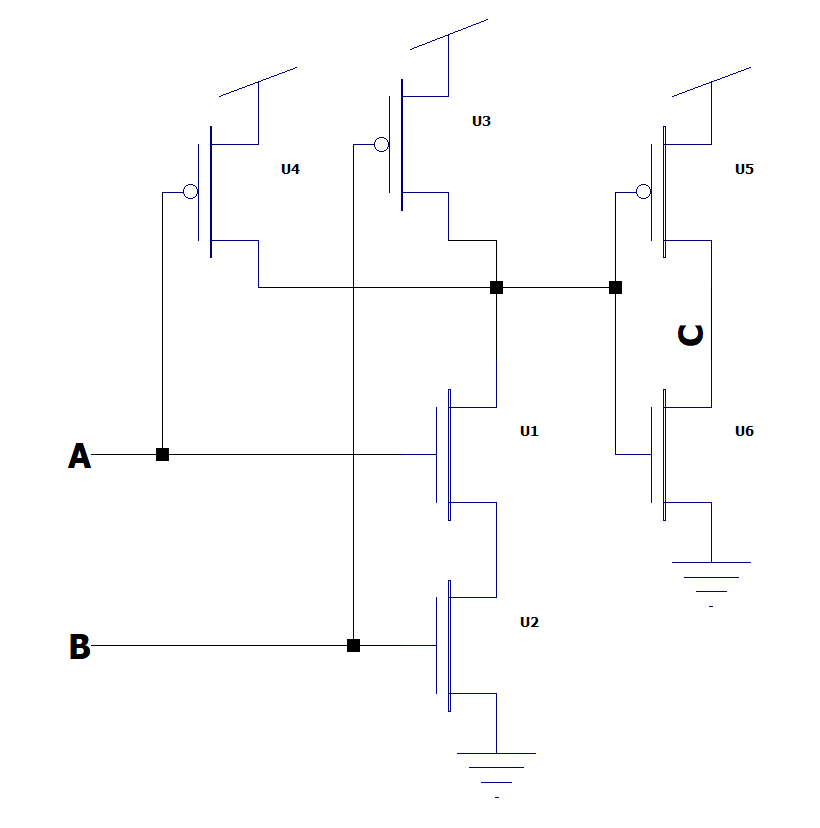
\includegraphics[scale = 0.5]{images/andgate.PNG}
  \caption{AND gate transistor-level schematic.}
  \label{fig:AND_schem}
  \end{center}
\end{figure}
% Description of how the gate level works at the transistor level
To make an AND gate, we connected both a NAND gate and and an inverter. The NAND gate, made up of the four leftmost transistors in Figure \ref{fig:AND_schem}, will return a low output when both inputs are high (because the two NMOS transistors will conduct and the two PMOS transistors will not conduct, so the overall output between them will be low) and return a high output in any other case (because at least one NMOS transistor will not conduct and at least one PMOS transistor will conduct, yielding a high output). Then, we connect the output of the NAND gate to an inverter (made up of the two rightmost transistors) - if the input to the inverter is low, then the PMOS transistor will be high and NMOS transistor will be low, resulting in a high output in between them. Conversely, if the output of the NAND gate is high, the NMOS transistor in the inverter will be high and the PMOS will be low, yielding a low output overall.

Combining the NAND gate and the inverter yields a device that outputs low if any of the inputs are low and outputs high if both inputs are high, which meets the expected functionality of an AND gate. 

We constructed the AND gate in LTspice and exhaustively tested it using the following test cases.
\begin{table}[h]
\begin{center}
 \begin{tabular}{|c c | c |} 
 \hline  
 Input &  & Expected Output \\
 \hline
 A & B & Output\\ 
 \hline
 0 & 0 & 0 \\ 
 \hline
 0 & 1 & 0 \\ 
 \hline
 1 & 0 & 0 \\ 
 \hline
 1 & 1 & 1 \\ 
 \hline
\end{tabular}
\caption{Test cases performed on AND gate.}
\end{center}
\end{table}

Our AND gate passed all of these tests, as illustrated in the plot below. The output is high if and only if both inputs are high, and otherwise the output is low. 

\begin{figure}[H]
  \begin{center}      
  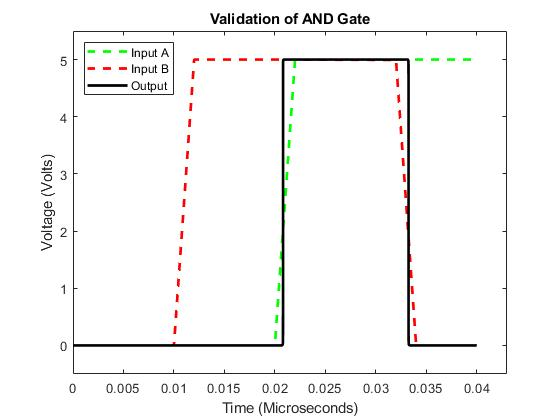
\includegraphics[scale = 0.5]{images/ANDplot.jpg}
  \caption{AND gate validation plot}   
  \label{fig:ANDplot}
  \end{center}
\end{figure}

\subsection{OR Gate}
We used CMOS components to construct an OR gate as shown in Figure \ref{fig:orgate}.

\begin{figure}[H]
  \begin{center}      
  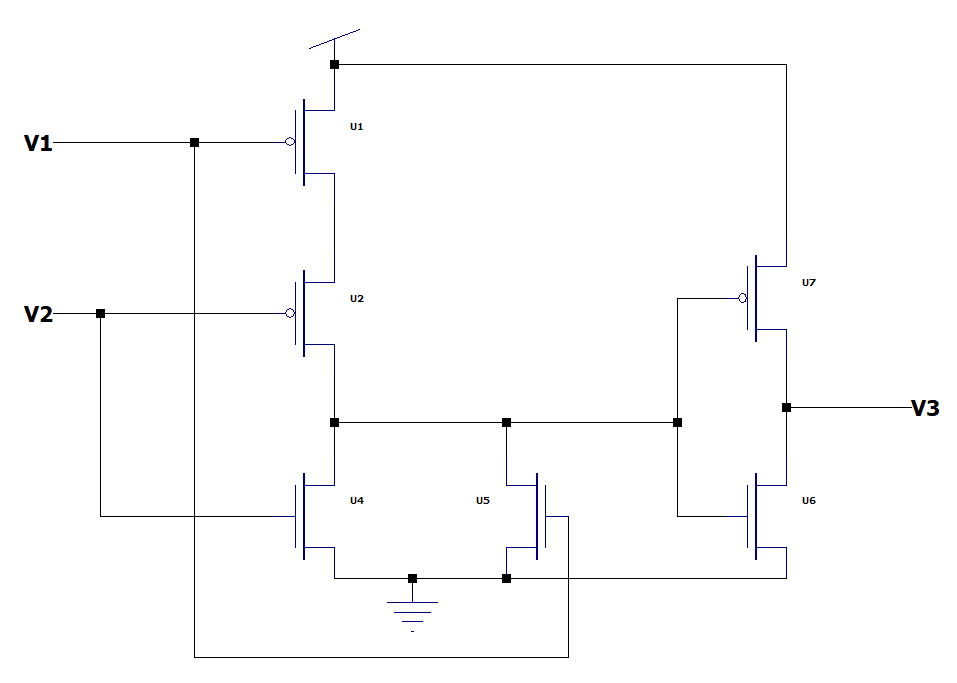
\includegraphics[scale = 0.5]{images/orgate.PNG}
  \caption{OR gate transistor-level schematic.}   
  \label{fig:orgate}
  \end{center}
\end{figure}

At the transistor level, the circuit consists of a few pieces that we can analyze: U1 and U2 make a PMOS NOR gate, U4 and U5 make an NMOS current mirror, and U6 and U7 make an inverter to turn the NOR gate output into OR gate logic.

In the PMOS NOR gate, when the gates of U1 and U2 are both held low, both PMOS transistors are on and current is allowed to flow. This makes the output of the NOR gate high. In the three other cases (U1 high and U2 low, U1 low and U2 high, or both gates high), at least one transistor is off which obstructs the flow of current and causes the output of the NOR gate to be low. 

When U1 and U2 are both low, the current mirror NMOS transistors are off. The current that flows through the NOR gate flows into the gates of U6 and U7. The inverter NMOS is on and the inverter PMOS is off, so Vout is low. 

When one of the inputs or both of the inputs is high, there is no current in the current mirror and the gates of the inverter transistors are pulled low. This means the inverter PMOS is on and the inverter NMOS is off, so the output is high in these three cases.


We constructed the OR gate in LTspice and exhaustively tested it using the following test cases.
\begin{table}[H]
\begin{center}
 \begin{tabular}{|c c | c |} 
 \hline  
 Input &  & Expected Output \\
 \hline
 A & B & Output\\ 
 \hline
 0 & 0 & 0 \\ 
 \hline
 0 & 1 & 1 \\ 
 \hline
 1 & 0 & 1 \\ 
 \hline
 1 & 1 & 1 \\ 
 \hline
\end{tabular}
\end{center}
\begin{center}
\caption{Test cases performed on OR Gate.}
\end{center}
\end{table}
Our OR gate passed all of these tests, as illustrated in the plot below. The output is low if and only if both inputs are low, and otherwise the output is high. 
% Plots
\begin{figure}[H]
  \begin{center}      
  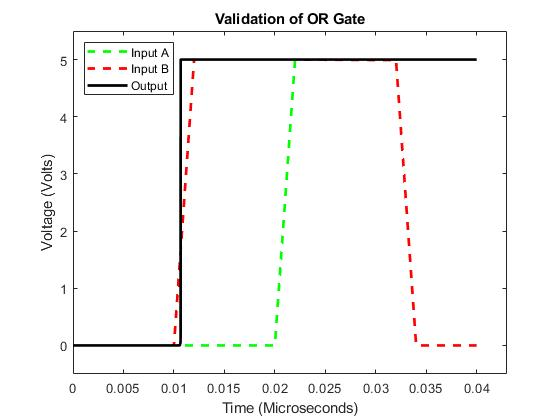
\includegraphics[scale = 0.5]{images/ORplot.jpg}
  \caption{OR gate validation plot.}   
  \label{fig:ORplot}
  \end{center}
\end{figure}


\subsection{XOR Gate}
We used CMOS components to construct an XOR gate.
\begin{figure}[H]
  \begin{center}      
  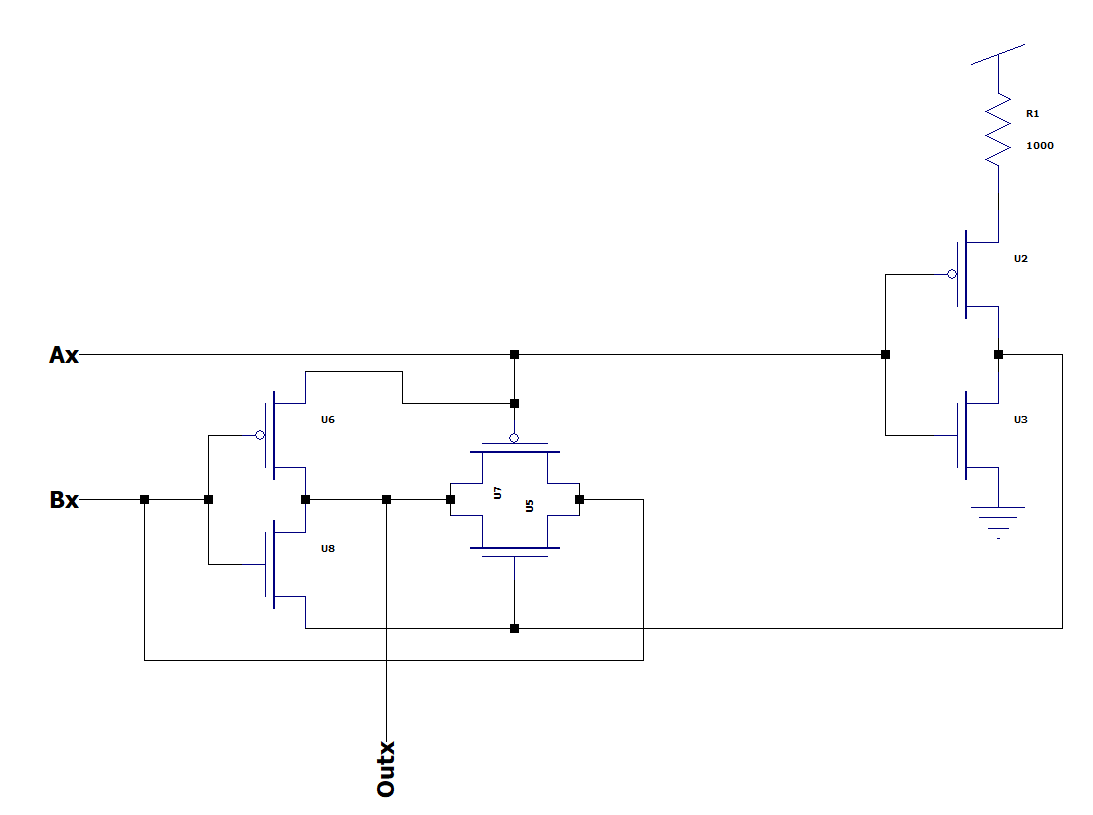
\includegraphics[scale = 0.5]{images/xorgate.PNG}
  \caption{XOR gate transistor-level schematic.}   
  \label{fig:exp1_schematic}
  \end{center}
\end{figure}

The XOR gate is made up of several parts: two inverters and an analog switch. The inverted and non-inverted forms of the Ax input are wired to the gates of the NMOS and PMOS analog switch transistors, respectively. The inverted and non-inverted forms of the Bx input are wired to the output of the whole circuit and the input to the analog switch, respectively.

When both Ax and Bx are low, the NMOS in the analog switch is on, and the PMOS in the switch is off. The switch passes the Bx input and drives the output low.

When Ax is high and Bx is low,  the NMOS and PMOS transistors in the analog switch are off. The Ax input powers the Bx inverter, which drives the output high. 

When Ax is low and Bx is high, the NMOS and PMOS transistors in the analog switch are on. The Bx inverter is not powered, and the analog switch passes the Bx input to the output so the output is high.

When both Ax and Bx are high, the NMOS and PMOS transistors in the analog switch are off. The Bx inverter is powered and Bx gets inverted, so the output is low.

We constructed the XOR gate in LTSpice and exhaustively tested it using the following test cases.
\begin{table}[H]
\begin{center}
 \begin{tabular}{|c c | c |} 
 \hline  
Input &  & Expected Output \\
 \hline
 A & B & Output\\ 
 \hline
 0 & 0 & 0 \\ 
 \hline
 0 & 1 & 1 \\ 
 \hline
 1 & 0 & 1 \\ 
 \hline
 1 & 1 & 0 \\ 
 \hline
\end{tabular}
\caption{Test cases beformed on XOR gate.}
\end{center}
\end{table}
% Plots 
Our XOR gate passed all of these tests, as illustrated on the plot below. The output is high if and only if both inputs are distinct, and otherwise the output is low. 

\begin{figure}[H]
  \begin{center}      
  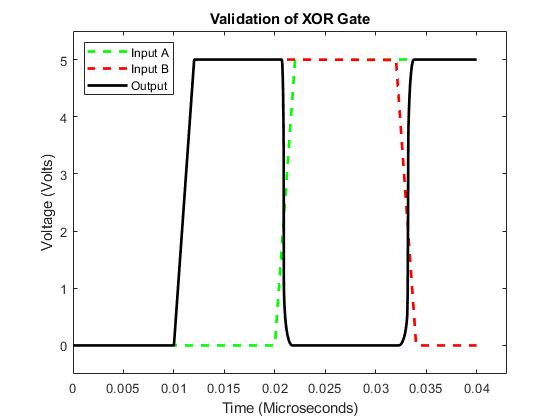
\includegraphics[scale = 0.5]{images/XORplot.jpg}
  \caption{XOR gate validation plot}   
  \label{fig:XORplot}
  \end{center}
\end{figure}

\section{One-Bit Adder}
Using combinations of the logic gates we developed, we created a one-bit adder. 
\begin{figure}[H]
  \begin{center}
  \includegraphics[scale = 0.5]{images/onebit.PNG}
  \caption{One-bit adder gate-level schematic.}   
  \label{fig:adder_schematic}
  \end{center}
\end{figure}
To calculate the sum bit, we use two cascaded XOR Gates. The first XOR gate determines the initial sum bit of the output based only on the inputs: if the inputs are both 0 or both 1, the initial sum will be 0, and if one is 0 and the other one is 1, the initial sum will be 1 (their sum). Then, if the carryin is equal to the initial sum, the output will be 0 (either reaffirming or adding to the original sum), and if the carryin is not equal to other original sum, it will effectively add 1 to the output.

To calculate the carryout, we AND each input together and we AND both the ouput and the carryin and then OR the results from those operations. This way, we can identify whether or not there is an overflow on the initial sum or after factoring in the carryin bit.

After constructing the adder using hierarchical schematics and our original logic gates, we exhaustively tested it to ensure it functioned in all possible cases.
\begin{table}[H]
\begin{center}
 \begin{tabular}{|c c c | c c |} 
 \hline  
 Input &  & & Expected Output & \\
 \hline
 A & B & Carryin & Sum & Carryout\\ 
 \hline
 0 & 0 & 0 & 0 & 0 \\ 
 \hline
 0 & 0 & 1 & 1 & 0 \\ 
 \hline
 0 & 1 & 0 & 1 & 1 \\ 
 \hline
 0 & 1 & 1 & 0 & 1 \\ 
 \hline
 1 & 0 & 0 & 1 & 0 \\ 
 \hline
 1 & 0 & 1 & 0 & 1 \\ 
 \hline
 1 & 1 & 0 & 0 & 1 \\ 
 \hline
 1 & 1 & 1 & 1 & 1 \\ 
 \hline 
\end{tabular}

\caption{Test cases performed on full one-bit adder.}

Our one-bit adder cell works with each possible set of inputs, as illustrated on the plot below.

\end{center}
\end{table}
\begin{figure}[H]
  \begin{center}      
  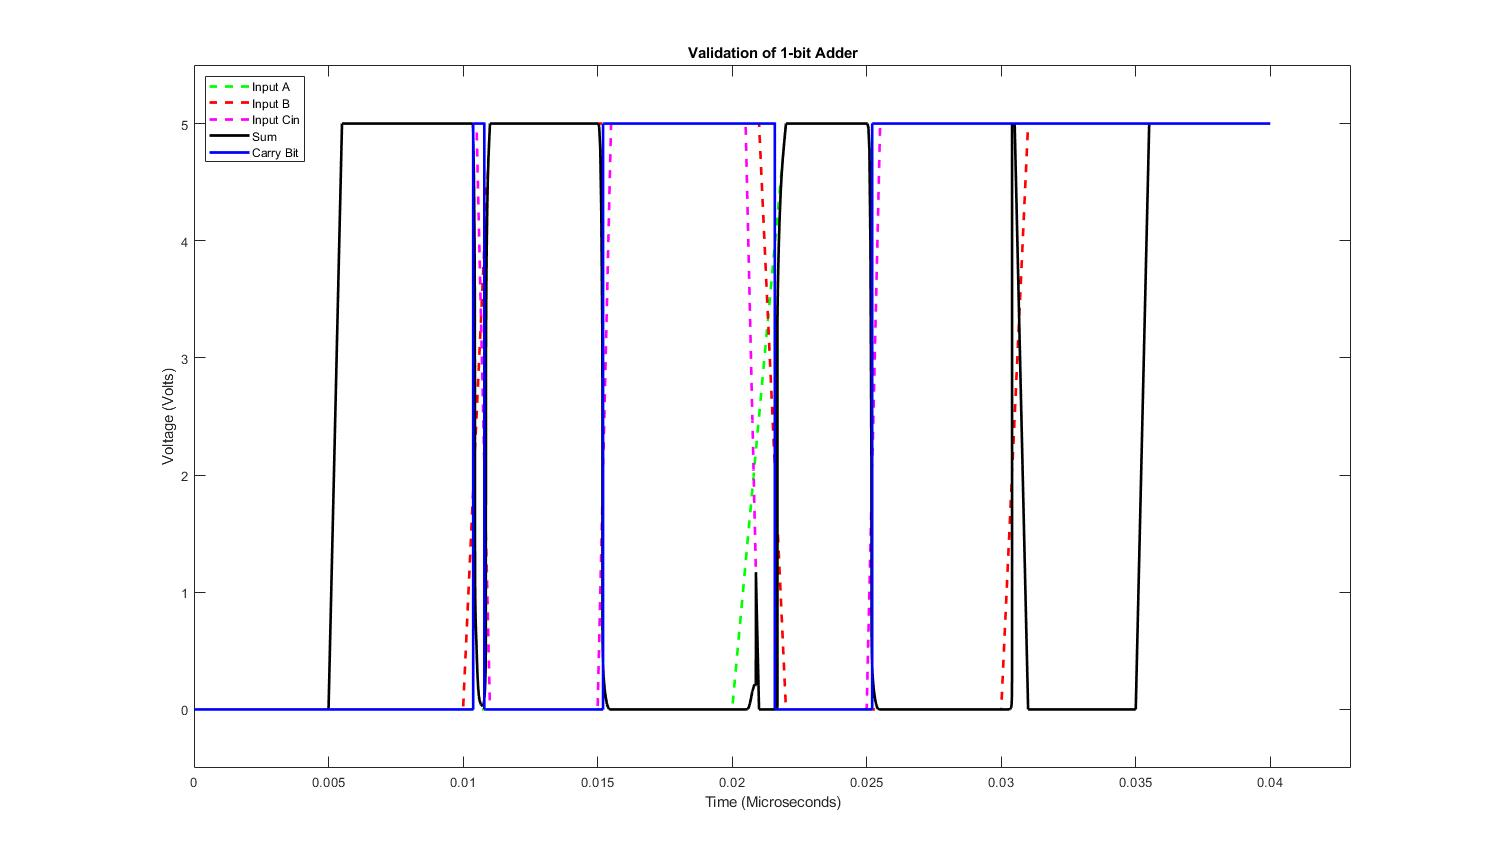
\includegraphics[width=0.9\textwidth]{images/1BITplot.jpg}
  \caption{One-bit adder validation plot}   
  \label{fig:ANDplot}
  \end{center}
\end{figure}


\section{Four-Bit Adder}
By connecting four of the one-bit adders that we developed, we created a four-bit adder. 
\begin{figure}[H]
  \begin{center}      
  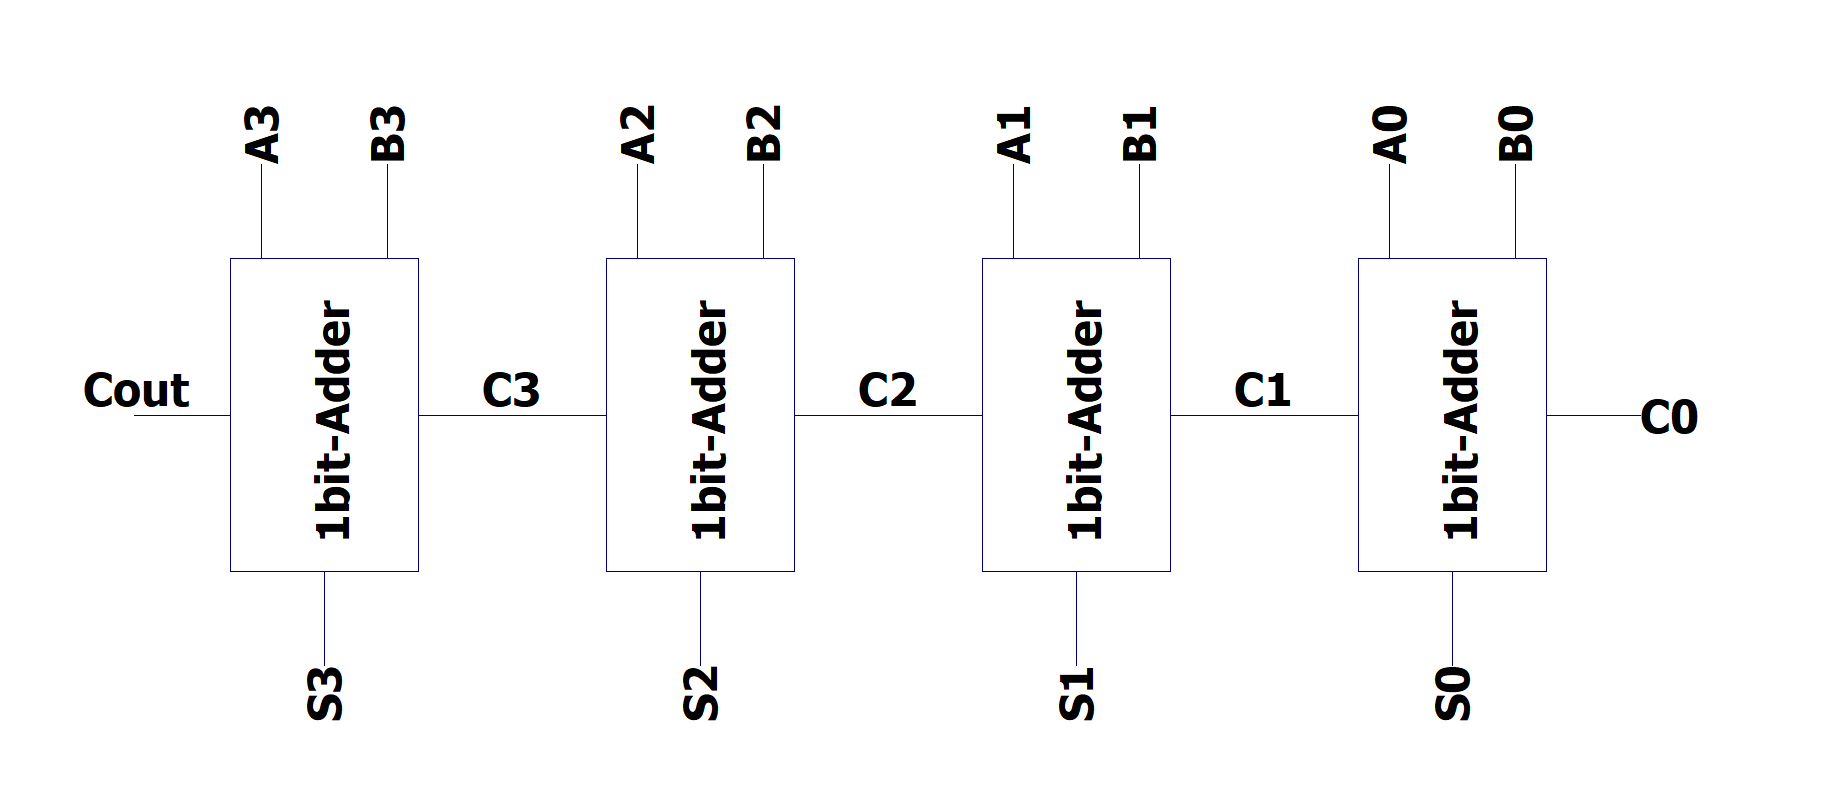
\includegraphics[width=0.8\textwidth]{images/fourbit.jpg}
  \caption{Four-bit ripple carry adder adder-level schematic}   
  \label{fig:adder_schematic}
  \end{center}
\end{figure}

To create the four-bit adder, we created a new one-bit adder for each bit of the binary representation of the two inputs. We then connected the carryout of each individual adder to the carryin of the adder for the following bit. This leaves a single input carryin and a single output carryout value associated with the final adder and a sum bit at each adder cell.

After assembling the four-bit adder in LTSpice, we created a test suite with the following cases to validate the functionality of carryin, carryout, and addition on each bit. By choosing these tests, we ensured we had high test coverage without having to exhaustively test all two hundred fifty-six possible cases.
\begin{table}[H]
\begin{center}
 \begin{tabular}{|c c c | c c |} 
 \hline  
 Input &  & & Expected Output & \\
 \hline
 A & B & Carryin & Sum & Carryout\\ 
 \hline
 0000 & 0000 & 0 & 0000 & 0 \\ 
 \hline
 0000 & 0000 & 1 & 0001 & 0 \\ 
 \hline
 1111 & 1111 & 0 & 1110 & 1 \\ 
 \hline
 1111 & 1111 & 1 & 1111 & 1 \\ 
 \hline
 1111 & 0000 & 0 & 1111 & 0 \\ 
 \hline
 1111 & 0000 & 1 & 0000 & 1 \\ 
 \hline
 0000 & 1111 & 0 & 1111 & 0 \\ 
 \hline
 0000 & 1111 & 1 & 0000 & 0 \\ 
 \hline 
\end{tabular}
\caption{Test cases performed on full four-bit adder.}
\end{center}
\end{table}
Our four-bit adder cell works with each set of inputs we tested from the cases above, as illustrated on the plot below. Because these tests validate each component of the adder, we feel confident that our device functions.
\begin{figure}[H]
  \begin{center}      
  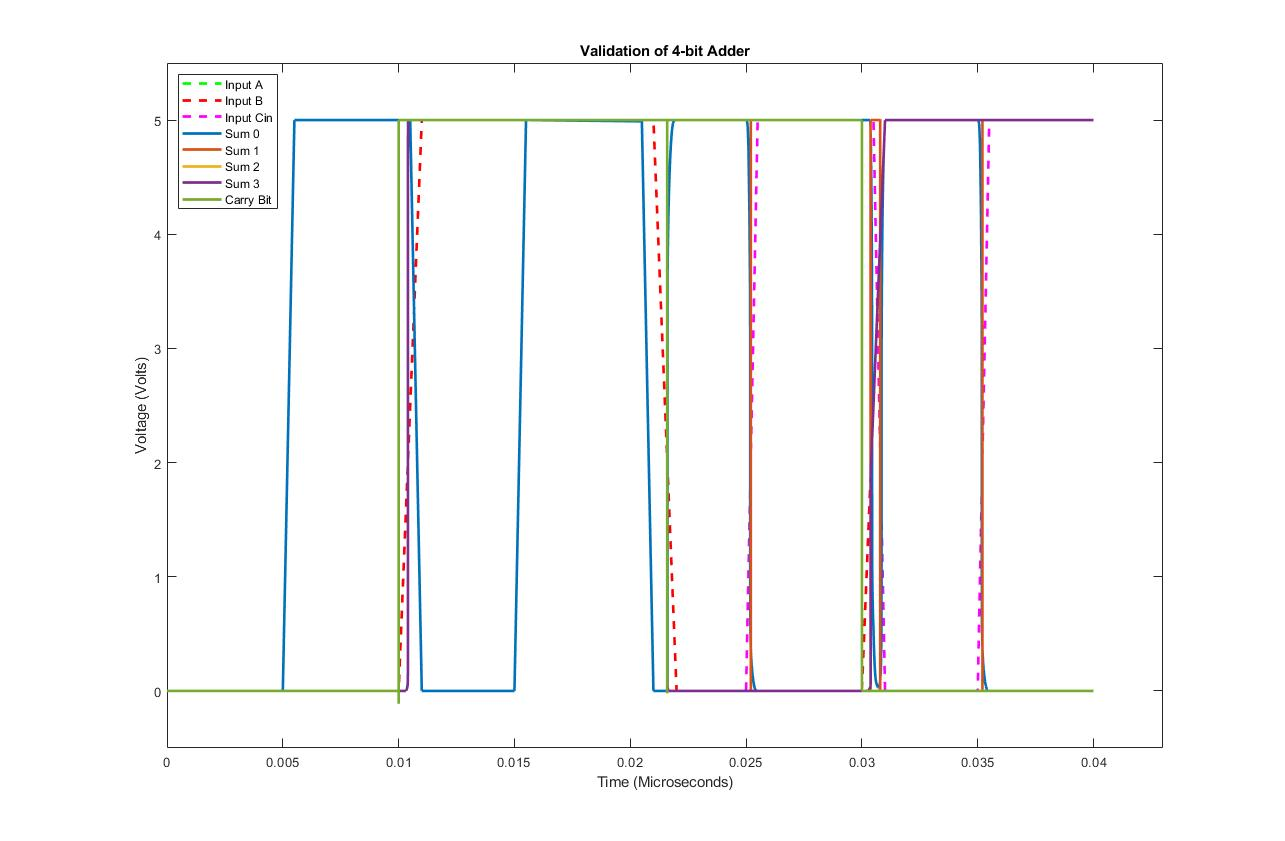
\includegraphics[width=0.9\textwidth]{images/4BITplot.jpg}
  \caption{Four-bit adder validation plot}   
  \label{fig:4bitplot}
  \end{center}
\end{figure}
\end{document}
